
\begin{frame}\frametitle{Summary}
\footnotesize\centering

\begin{minipage}{.7\textwidth}\centering

Discussed two searches for heavy top partners in the single lepton channel, using 14~\ifb\ of $pp$ data at \rts=8~\tev

\myskip

\begin{minipage}{.4\textwidth}\centering

\includegraphics[width=.9\textwidth]{pics/combo/lim_Scan2D_comb.pdf}

\end{minipage}\begin{minipage}{.5\textwidth}\centering

\begin{itemize}
\item Complementary
\item Model-independent
\item Sensitive to ``general'' new physics
\end{itemize}

\end{minipage}


\end{minipage}

\myskip

\begin{minipage}{.2\textwidth}\centering
\includegraphics[width=1.\textwidth]{pics/VLQAna_WbX_1W_MWb_4_ELEMUON_cutflow1234567_NOMINAL.pdf}
\end{minipage}\begin{minipage}{.3\textwidth}\centering

\scriptsize

\begin{itemize}
\item Optimal for $\TTbar\to WbWb$
\end{itemize}

Best up-to-date 95\% CL obs limit on 
chiral $T$ and vector-like $Y$ (740~\gev)

\end{minipage}\begin{minipage}{.2\textwidth}\centering

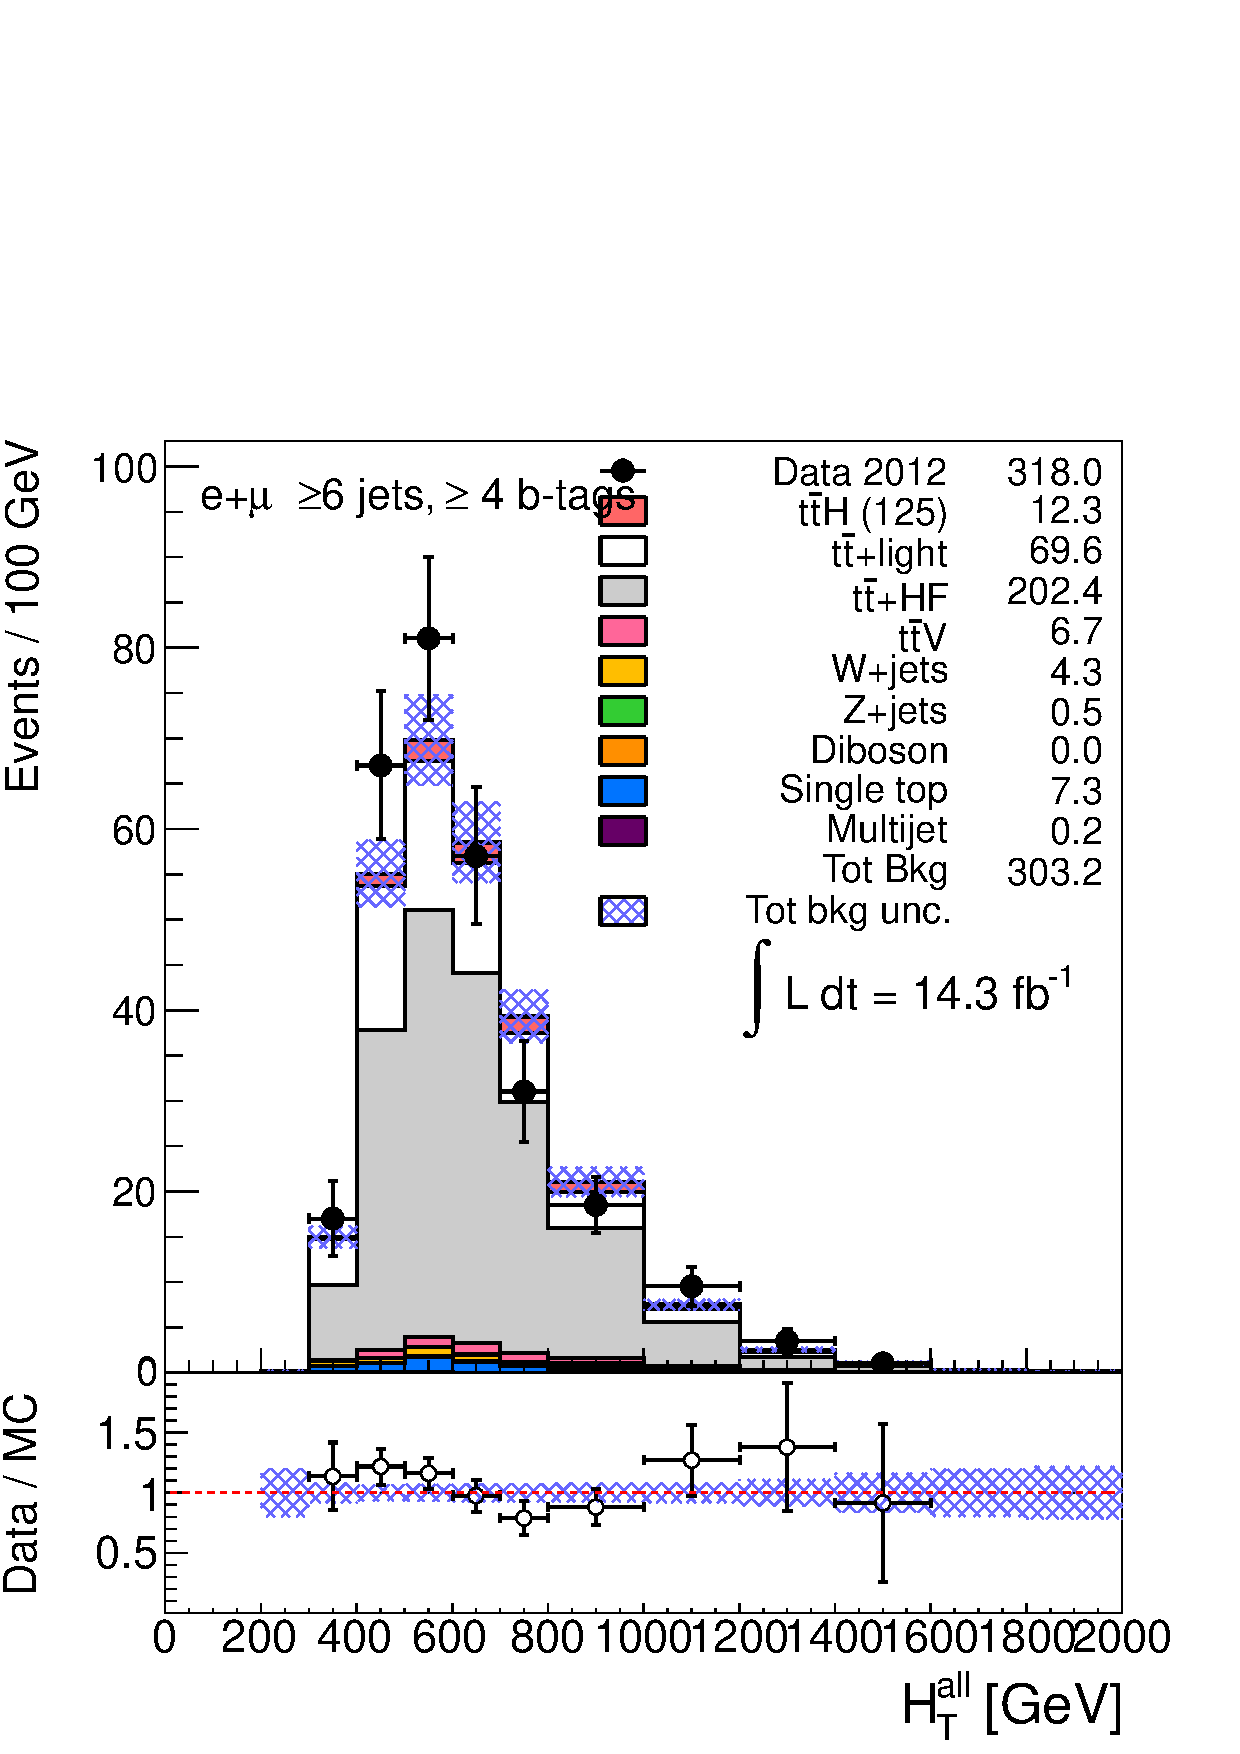
\includegraphics[width=1.\textwidth]{pics/htx_final/HTAll_6jetin4btagin_ELEMUON.pdf}

\end{minipage}\begin{minipage}{.3\textwidth}\centering

\scriptsize
\begin{itemize}
\item Optimal for $\TTbar\to HtX$
\end{itemize}

Best up-to-date 95\% CL obs limit on doublet $T$

\end{minipage}

\end{frame}


\begin{frame}\frametitle{Conclusions and short-term outlook}
\footnotesize\centering

{\it all ATLAS searches are being updated with the full {\cccolor 20~\ifb} statistics}\\ plus two new channels: $B\bar{B}\to Wt+X$ and $B\bar{B}\to Hb+X$

\begin{minipage}{.3\textwidth}\centering
\includegraphics[width=.7\textwidth]{pics/VLQAna_WbX_1W_MWb_4_ELEMUON_cutflow1234567_NOMINAL.pdf}
\end{minipage}\begin{minipage}{.7\textwidth}\centering
\begin{tabular}{l}
\buuu poor MC bkgs statistical population in the \tight\ channel\\
\\
\yeee {\cccolor larger MC samples} available\\
\yeee possible optimization of the {\cccolor\htfj\ cut}\\
\yeee explorable option: larger anti-$k_{t}$ {\cccolor jets}\\
\end{tabular}

\end{minipage}

\begin{minipage}{.7\textwidth}\centering
\begin{tabular}{l}
\buuu poor modeling of \tthf\ by \texttt{ALPGEN}\\
\buuu \btag ging calibration sub-optimal for\\
\phantom{\buuu} analyses with high-\pt\ objects\\
\\
\yeee {\cccolor\ttbar-based} calibrations being developed\\
\yeee potential high gain in sensitivity with {\cccolor profiling}\\
\yeee easily optimizable for a {\cccolor$B\bar{B}\to Hb+X$} analysis\\
\end{tabular}

\end{minipage}\begin{minipage}{.3\textwidth}\centering
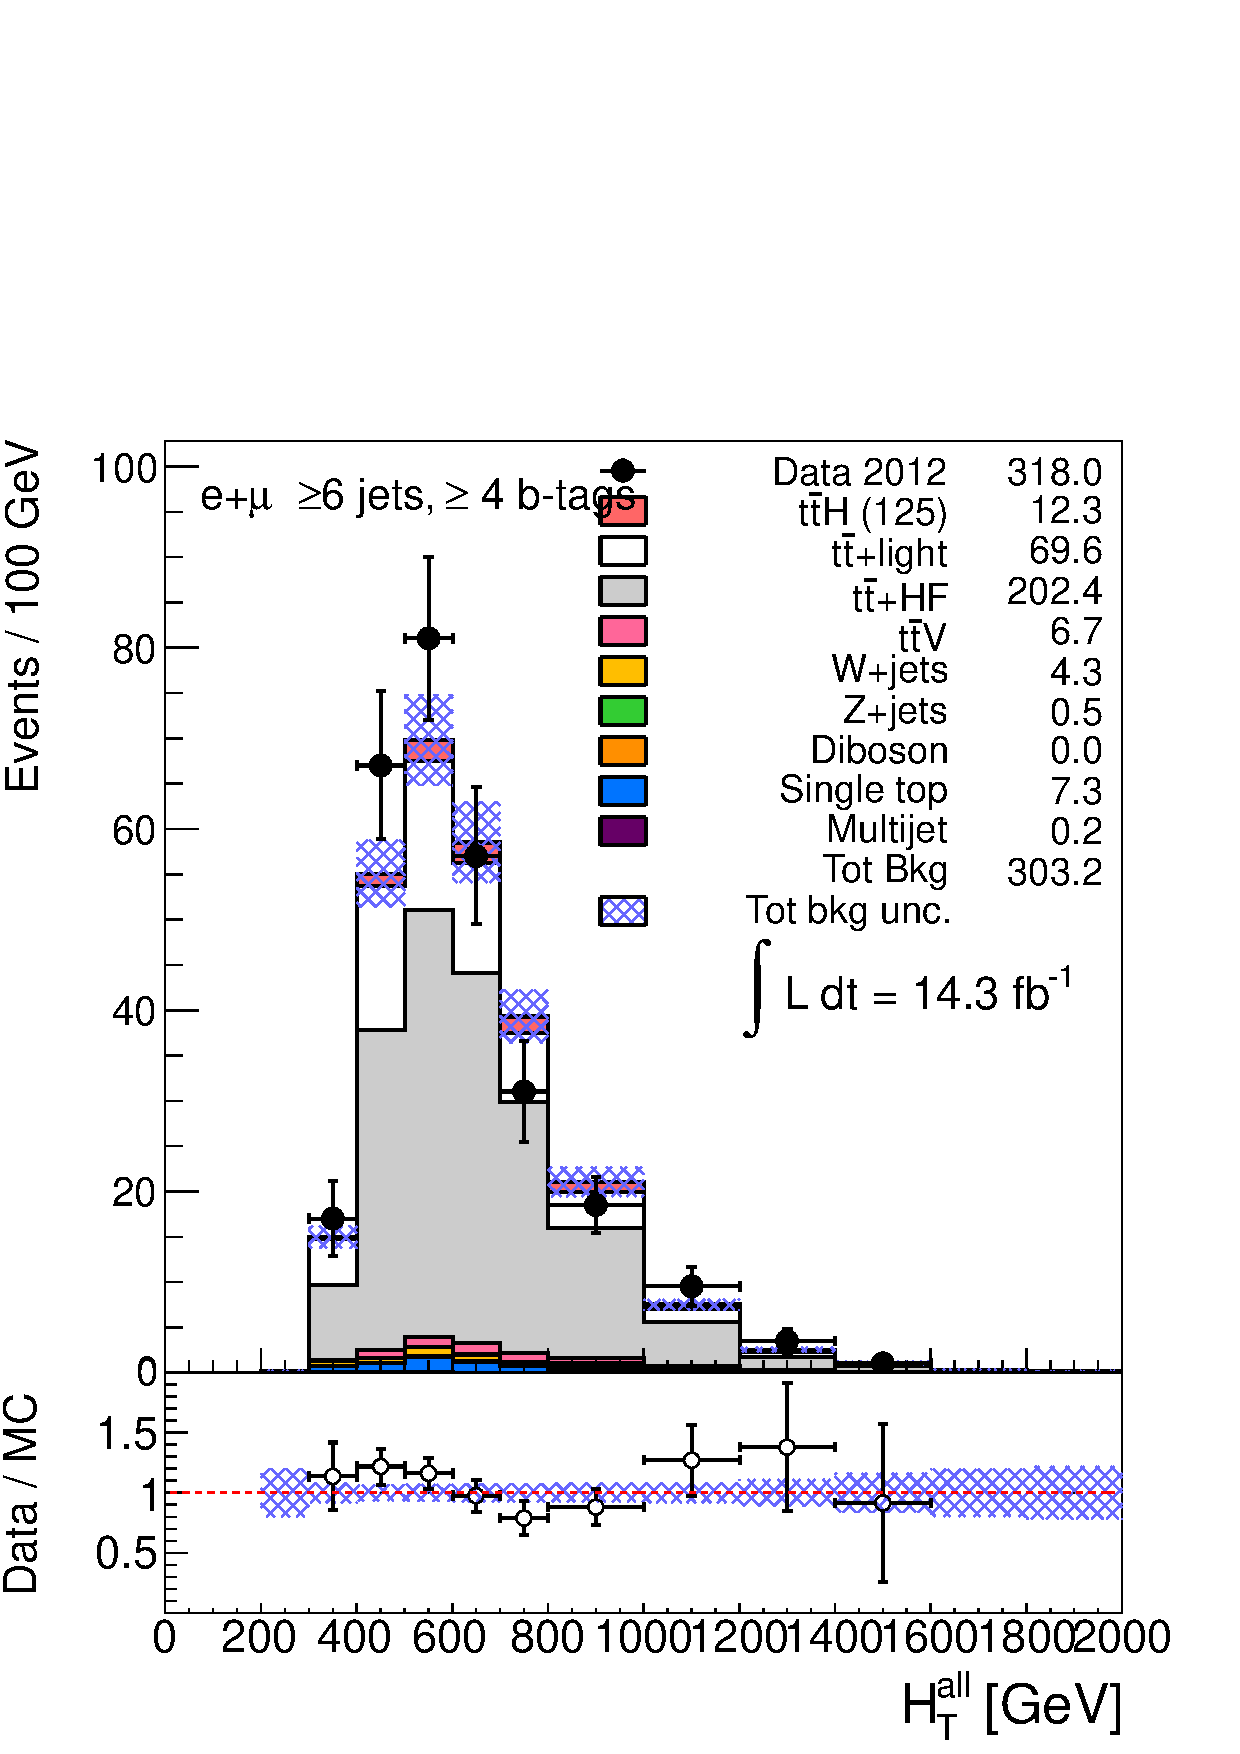
\includegraphics[width=.7\textwidth]{pics/htx_final/HTAll_6jetin4btagin_ELEMUON.pdf}
\end{minipage}

\end{frame}

\begin{frame}\frametitle{``Long''-term outlook}
\small\centering


\begin{pgfpicture}{0.0\textwidth}{0.0\textheight}{1.\textwidth}{.35\textwidth}
%   \begin{pgftranslate}{\pgfpoint{0.05\textwidth}{-0.12\textheight}}
%   \end{pgftranslate}
\pgfdeclareimage[interpolate=true,width=.45\textwidth]{xsec13}{pics/ja/fig4b}
\pgfdeclareimage[interpolate=true,width=.45\textwidth]{xsec8}{pics/ja/fig4a}
\pgfputat{\pgfxy(0.0,0.)}{\pgfbox[left,base]{\pgfuseimage{xsec8}}}
\pgfputat{\pgfxy(6.5,0.)}{\pgfbox[left,base]{\pgfuseimage{xsec13}}}
 {\usebeamercolor[fg]{head/foot boxes}
 \pgfline{\pgfxy(7.9,0.4)}{\pgfxy(7.9,3.05)}
 \pgfline{\pgfxy(7.,3.05)}{\pgfxy(7.9,3.05)}
 \pgfline{\pgfxy(0.5,2.86)}{\pgfxy(1.42,2.86)}
 \pgfline{\pgfxy(1.42,0.4)}{\pgfxy(1.42,2.9)}
 }
\end{pgfpicture}

\myskip

\begin{minipage}{.4\textwidth}\centering
LHC Run-II: \\
\myskip
\begin{tabular}{l}
\yeee \rts=14~\tev\\
\yeee $\sim 100\ifb$ in 3 years\\
\buuu higher pile-up\\
\end{tabular}

\end{minipage}\begin{minipage}{.6\textwidth}\centering

To-do:\\
\begin{itemize}
\item continue on the road of full combination
\item design searches for single production
\end{itemize}

\end{minipage}

\begin{flushright}\scriptsize
plots from~\cite{Aguilar-Saavedra:2013qpa}
\end{flushright}

\end{frame}


\begin{frame}\frametitle{Thank you!}
\large\centering


Thank you for your attention!

\myskip

\includegraphics[width=.5\textwidth]{pics/boooks.jpg}

\end{frame}
